\documentclass[a4paper, 8pt, twoside, openright]{book}
\usepackage[a4paper,top=4cm,bottom=2cm,left=2cm,right=2cm]{geometry}
\usepackage[english]{babel}
\usepackage[T1]{fontenc}
\usepackage[utf8]{inputenc}
\usepackage{fancyhdr}
\usepackage{float}
\usepackage{graphicx}
\usepackage{wrapfig}
\usepackage{siunitx} %per scrivere il simbolo °
\usepackage{verbatim} %per i commenti1
\usepackage{subfig}
\usepackage{amsmath}
\usepackage{algorithm}
\usepackage{algpseudocode}
\setcounter{secnumdepth}{3}
\setcounter{tocdepth}{6}
\usepackage{multirow}
\newcommand{\minitab}[2][l]{\begin{tabular}#1 #2\end{tabular}}
\usepackage{rotating}
\usepackage{xfrac}

\DeclareMathOperator*{\argmax}{arg\,max}
\DeclareMathOperator*{\argmin}{arg\,min}

%\usepackage{booktabs,array}
%\usepackage{tikz}

%\usepackage{tabularx}

%\usepackage{chngcntr}
%\counterwithin{table}{section}

%------------------------------ colors
\usepackage[usenames,dvipsnames,table]{xcolor} % use colors on table and more
\definecolor{333}{RGB}{51, 51, 51} % define custom color
\definecolor{background}{RGB}{248, 248, 255}
\definecolor{comment}{RGB}{17,167,5}
\definecolor{keyword}{RGB}{195,47,8}
\definecolor{string}{RGB}{142,195,0}
\definecolor{number}{RGB}{90,84,84}
\definecolor{identifier}{RGB}{0,90,201}

%------------------------------ source code
\usepackage{listings}

\lstset{
  basicstyle=\footnotesize\sffamily,
  commentstyle=\itshape\color{gray},
  captionpos=b,
  frame=shadowbox,
  language=HTML,
  rulesepcolor=\color{333},
  tabsize=2
}

\lstdefinestyle{code}{
  backgroundcolor=\color{background},
  basicstyle=\footnotesize\sffamily,
  commentstyle=\color{comment},
  frame=L,
  identifierstyle=\color{identifier},
  keywordstyle=\color{keyword},
  numbers=left,
  numbersep=10pt,
  numberstyle=\tiny\color{number},
  stringstyle=\color{string},
  showstringspaces=false,  
  stepnumber=1,
  tabsize=2
}


%------------------------------ define Abstract environment, missing in the 'book' class
\newenvironment{abstract}{\cleardoublepage \null \vfill \begin{center}\bfseries\abstractname \end{center}}{\vfill\null}
\addto\captionsenglish{\renewcommand*\abstractname{Abstract}} % change Abstract title

%------------------------------ active url
\usepackage{url}
\renewcommand{\UrlFont}{\color{black}\small\ttfamily}
\usepackage[colorlinks=true, linkcolor=black, citecolor=black, urlcolor=black]{hyperref} % active ref
%------------------------------ macros
\newcommand{\sectionname}{Section} % define Section ref
\newcommand{\subsectionname}{Sub-section} % define Sub-section ref
\renewcommand*\arraystretch{1.4} % tables padding

%acronimi
\usepackage[printonlyused]{acronym}

\begin{document}
\frontmatter

\begin{titlepage} %------------------------------ TITLE PAGE
\begin{center}
\vbox to0pt{\vbox to\textheight{\vfill 
\includegraphics[width=11.5cm]{./Images/Background} \vfill}\vss}

\begin{center}
\begin{minipage}{.20\textwidth}
  
\includegraphics[height=2.5cm]{./Images/Icon4}
\end{minipage}\begin{minipage}{.45\textwidth}
  \begin{table}[H]
  \begin{tabular}{l}
  \scshape{\Large{\bfseries{Padua University}}} \\
  \hline \\
  \scshape{\Large{Engineering Course}} \\
  \end{tabular}
  \end{table}
\end{minipage}
\end{center}


\vspace{1cm}
\emph{\Large{Master~of~Computer~Engineering}} \\
\vspace{0.9cm}
\scshape{\Large{\bfseries{Computer Networks}}} \\
\vspace{0.2cm} \linespread{1} \scshape{\large{\bfseries{}}}
\end{center}

\vspace{12cm}
\begin{center}
Raffaele Di Nardo Di Maio
\end{center}

\vfill
\begin{center}
\hspace{-0.2cm}
\line(1, 0){360}\\
\textsc{Accademic Year 2019-2020}
\end{center}
\end{titlepage}


\cleardoublepage % make left page blank
\thispagestyle{empty} %------------------------------ DEDICA

\begin{comment}
\null
\vspace{2cm}
\begin{flushright}
//DEDICA
\end{flushright}
\vfill
\begin{quote}
  \textit{}
\end{quote}
\vfill
\null
\end{comment}

%\begin{abstract} %------------------------------ ABSTRACT
%\addcontentsline{toc}{chapter}{Abstract}
%\markboth{}{} % remove header
%\thispagestyle{empty}
%This is the abstract
%\end{abstract}

%\input{Chapters/Abstract.tex}
\begingroup %------------------------------ CONTENTS
  \makeatletter
  \let\ps@plain\ps@empty
  \makeatother
  \tableofcontents  
  \clearpage
\endgroup

\mainmatter
\chapter{C programming}
The C is the most powerful language and also can be considered as the language nearest to Assembly language. Its power is the speed of execution and the easy interpretation of the memory.\\
C can be considered very important in Computer Networks because it doesn't hide the use of system calls. Other languages made the same thing, but hiding all the needs and evolution of Computer Network systems.

\section{Organization of data}\label{littleBig}
Data are stored in the memory in two possible ways, related to the order of bytes that compose it. There are two main ways, called Big Endian and Little Endian.
\begin{center}
\begin{tabular}{c}
\begin{lstlisting}[linewidth=30pt, basicstyle=\footnotesize\sffamily,]
int i;
\end{lstlisting}
\end{tabular}
\end{center}

\begin{figure}[h]
\centering
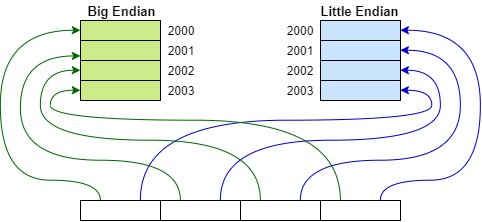
\includegraphics[scale=0.68]{Images/Programming/endians}
\caption{\footnotesize{Little Endian and Big Endian.}}
\end{figure}

The order of bytes in packets, sent through the network, is Big Endian.\\
The size of \textbf{int, float, char, ...} types
depends on the architecture used. The max size of possible types depends on the architecture (E.g. in 64bits architecture, in one istruction, 8 bytes can be written and read in parallel).

\begin{table}[h]
\centering
\begin{tabular}{|c|c|}
\hline
\textbf{signed}&{unsigned}\\
\hline
{int8\_t}&{uint8\_t}\\
{int16\_t}&{uint16\_t}\\
{int32\_t}&{uint32\_t}\\
{int64\_t}&{uint64\_t}\\
\hline
\end{tabular}\caption{<stdint.h>}
\end{table}
\vspace{4cm}
\section{Struct organization of memory}
The size of a structure depends on the order of fields and the architecture. This is caused by alignment that depends on the number of memory banks, number of bytes read in parallel. For example the size is 4 bytes for 32 bits architecture, composed by 4 banks (Figure \ref{parallel}). The Network Packet Representation is made by a stream of 4 Bytes packets as we're using 32 bits architecture. 
\begin{center}
\begin{tabular}{c}
\begin{lstlisting}[linewidth=200pt, basicstyle=\footnotesize\sffamily,]
struct example1        struct example2
{                      {
	char c;	               int x;
	int x;	               char c;
}                      }
\end{lstlisting}
\end{tabular}
\end{center}

\begin{figure}[h]
\centering
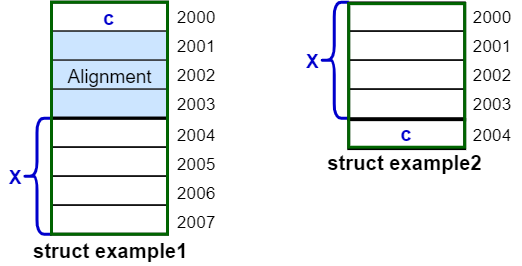
\includegraphics[scale=0.5]{Images/Programming/struct}
\end{figure}

\begin{figure}[h]
\centering
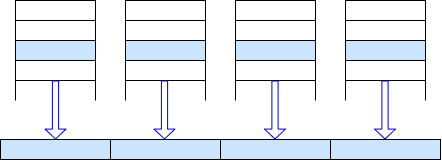
\includegraphics[scale=0.68]{Images/Programming/parallel_reading}
\caption{\footnotesize{Parallel reading in one istruction in 32 bits architecture.}}\label{parallel}
\end{figure}

\vspace{3cm}
\section{Structure of C program}
The program stores the variable in different section (Figure \ref{program}):
\begin{itemize}
\item{\textbf{Static area}\\
where global variables and static library are stored, it's initialized immediately at the creation of the program. Inside this area, a variable doesn't need to be initialized by the programmer because it's done automatically at the creation of the program with all zeroes.}
\item{\textbf{Stack}\\
allocation of variables, return and parameters of functions}
\item{\textbf{Heap}\\
dinamic allocation }
\end{itemize}

\begin{figure}[h]
\centering
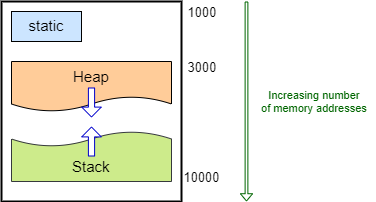
\includegraphics[scale=0.68]{Images/Programming/program}
\caption{\footnotesize{Structure of the program.}}\label{program}
\end{figure}
\chapter{Network services in C}
\section{Application layer}
We need IP protocol to use Internet. In this protocol, level 5 and 6 are hidden in Application Layer.\\
In this case, Application Layer needs to interact with Transport Layer, that is implemented in OS Kernel (Figure \ref{app_kernel}). Hence Application and Transport can talk each other with System Calls.
\begin{figure}[h]
\centering
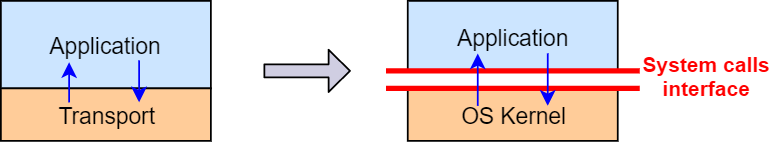
\includegraphics[scale=0.6]{Images/NetworkC/application}\caption{\footnotesize{System calls interface.}}\label{app_kernel}
\end{figure}

\section{socket}\label{socket}
Entry-point (system call) that allow us to use the network services. It also allows application layer to access to level 4 of IP protocol. 
\begin{center}
\begin{tabular}{c}
\begin{lstlisting}[linewidth=270pt, basicstyle=\footnotesize\sffamily,]
#include <sys/types.h>
#include <sys/socket.h>

int socket(int domain, int type, int protocol);\\
\end{lstlisting}
\end{tabular}
\end{center}

\begin{table}[h]
\centering
\begin{tabular}{rcl}
\textbf{RETURN VALUE} & \multicolumn{2}{l}{\textit{File Descriptor (FD) of the socket} }\\
{} & \multicolumn{2}{l}{\textit{-1} if some error occurs and errno is set appropriately}\\
{} & \multicolumn{2}{l}{(You can check value of errno including <errno.h>).}\\
\end{tabular}
\end{table}

\begin{table}[h]
\centering
\begin{tabular}{rcl}
\textbf{domain =} & \multicolumn{2}{l}{\textit{Communication domain}}\\
{} & \multicolumn{2}{l}{protocol family which will be used for communication.}\\
{} & \textbf{AF\_INET:} & {IPv4 Internet Protocol}\\
{} & \textbf{AF\_INET6:} & {IPv6 Internet Protocol}\\
{} & \textbf{AF\_PACKET:} & {Low level packet interface}\\
& &\\
\textbf{type =} & \multicolumn{2}{l}{\textit{Communication semantics}}\\
{} & \textbf{SOCK\_STREAM:} & {Provides sequenced, reliable, two-way, connection-based}\\
{} & {} & {bytes stream. An OUT-OF-BAND data mechanism may}\\
{} & {} & {be supported.}\\
{} & \textbf{SOCK\_DGRAM} & {Supports datagrams (connectionless, unreliable messages} \\
& & {of a fixed maximum length).}\\
& & \\
\textbf{protocol =} & \multicolumn{2}{l}{\textit{Particular protocol to be used within the socket}}\\
{} & \multicolumn{2}{l}{Normally there is only a protocol for each socket type and protocol}\\
{} & \multicolumn{2}{l}{family (protocol=0), otherwise ID of the protocol you want to use}\\
\end{tabular}
\end{table}

\vspace{10cm}
\section{TCP connection}
In TCP connection, defined by type \textbf{SOCK\_STREAM} as written in the Section \ref{socket}, there is a client that connects to a server. It uses three primitives (related to File System primitives for management of files on disk) that do these logic actions:
\begin{enumerate}
\item{start (open bytes stream)}
\item{add/remove bytes from stream}
\item{finish (clos bytes stream)}
\end{enumerate}
TCP is used transfering big files on the network and for example with HTTP, that supports parallel download and upload (FULL-DUPLEX). The length of the stream is defined only at closure of the stream.
 
\subsection{Client}
\subsubsection{connect}
The client calls \textbf{connect()} function, after \textbf{socket()} function of Section \ref{socket}. This function is a system call that client can use to define what is the remote terminal to which he wants to connect.

\begin{center}
\begin{tabular}{c}
\begin{lstlisting}[linewidth=370pt, basicstyle=\footnotesize\sffamily,]
#include <sys/types.h>
#include <sys/socket.h>

int connect(int sockfd, const struct sockaddr *addr,socklen_t addrlen);
\end{lstlisting}
\end{tabular}
\end{center}

\begin{table}[h]
\centering
\begin{tabular}{rcl}
\textbf{RETURN VALUE} & \multicolumn{2}{l}{\textit{0} if connection succeds}\\
{} & \multicolumn{2}{l}{\textit{-1} if some error occurs and errno is set appropriately}\\
& & \\
\textbf{sockfd =} & \multicolumn{2}{l}{\textit{Socket File Descriptor} returned by socket().}\\
& &\\
\textbf{addr =} & \multicolumn{2}{l}{\textit{Reference to struct sockaddr}}\\
{} & \multicolumn{2}{l}{sockaddr is a general structure that defines the concept of address.}\\
{} & \multicolumn{2}{l}{In practice it's a union of all the possible specific structures of each protocol.}\\
{} & \multicolumn{2}{l}{This approach is used to leave the function written in a generic way.}\\
& & \\
\textbf{addr =} & \multicolumn{2}{l}{\textit{Length of specific data structure used.}}\\
\end{tabular}
\end{table}
\vspace{8cm}
In the following there is the description of struct \textbf{sockaddr\_in}, that is the specific sockaddr structure implemented for family of protocls \textbf{AF\_INET}:

\begin{center}
\begin{tabular}{c}
\begin{lstlisting}[linewidth=350pt, basicstyle=\footnotesize\sffamily,]
#include <netinet/in.h>

struct sockaddr_in {
    sa_family_t    sin_family; /* address family: AF_INET */
    in_port_t      sin_port;   /* port in network byte order */
    struct in_addr sin_addr;   /* internet address */
};

/* Internet address. */
struct in_addr {
    uint32_t       s_addr;     /* address in network byte order */
};\\
\end{lstlisting}
\end{tabular}
\end{center}
As mentioned in Section \ref{littleBig}, network data are organized as Big Endian, so in this case we need to insert the IP address according to this protocol. It can be done as in previous example or with the follow function:
\begin{center}
\begin{tabular}{c}
\begin{lstlisting}[linewidth=280pt, basicstyle=\footnotesize\sffamily,]
#include <sys/socket.h>
#include <netinet/in.h>
#include <arpa/inet.h>

int inet_aton(const char *cp, struct in_addr *inp);
\end{lstlisting}
\end{tabular}
\end{center}
The port number is written according to Big Endian architecture, through the next function:
\begin{center}
\begin{tabular}{c}
\begin{lstlisting}[linewidth=200pt, basicstyle=\footnotesize\sffamily,]
#include <arpa/inet.h>

uint16_t htons(uint16_t hostshort);
\end{lstlisting}
\end{tabular}
\end{center}

\subsubsection{write()}
Application protocol uses a readable string, to excange readable information (as in HTTP). This tecnique is called simple protocol and commands, sent by the protocol, are standardized and readable strings.  

\begin{center}
\begin{tabular}{c}
\begin{lstlisting}[linewidth=280pt, basicstyle=\footnotesize\sffamily,]
#include <unistd.h>

ssize_t write(int fd, const void *buf, size_t count);
\end{lstlisting}
\end{tabular}
\end{center}

\begin{table}[h]
\centering
\begin{tabular}{rcl}
\textbf{RETURN VALUE} & \multicolumn{2}{l}{\textit{Number of bytes written} on success}\\
{} & \multicolumn{2}{l}{\textit{-1} if some error occurs and errno is set appropriately}\\
& & \\
\textbf{fd =} & \multicolumn{2}{l}{\textit{Socket File Descriptor} returned by socket().}\\
& &\\
\textbf{buf =} & \multicolumn{2}{l}{\textit{Buffer of characters to write}}\\
& & \\
\textbf{count =} & \multicolumn{2}{l}{\textit{Max number of bytes to write} in the file (stream).}\\
\end{tabular}
\end{table}
\vspace{4cm}
The write buffer is usually a string but we don't consider the null value (\textbf{$\backslash 0$} character), that determine the end of the string, in the evaluation of count (\textbf{strlen(buf)-1}). This convention is used because \textbf{$\backslash 0$} can be part of characters stream.\\

\subsubsection{read()}
The client uses this blocking function to wait and obtain response from the remote server. Not all the request are completed immediat from the server, for the meaning of stream type of protocol. Infact in this protocol, there is a flow for which the complete sequence is defined only at the closure of it\ref{socket}.\\
\textbf{read()} is consuming bytes fom the stream asking to level 4 a portion of them, because it cannot access directly to bytes in Kernel buffer. Lower layer controls the stream of information that comes from the same layer of remove system.\\

\begin{center}
\begin{tabular}{c}
\begin{lstlisting}[linewidth=280pt, basicstyle=\footnotesize\sffamily,]
#include <unistd.h>

       ssize_t read(int fd, void *buf, size_t count);
\end{lstlisting}
\end{tabular}
\end{center}

\begin{table}[h]
\centering
\begin{tabular}{rcl}
\textbf{RETURN VALUE} & \multicolumn{2}{l}{\textit{Number of bytes read} on success}\\
{} & \multicolumn{2}{l}{\textit{0} if EOF is reached (end of the stream)}\\
{} & \multicolumn{2}{l}{\textit{-1} if some error occurs and errno is set appropriately}\\
& & \\
\textbf{fd =} & \multicolumn{2}{l}{\textit{Socket File Descriptor} returned by socket().}\\
& &\\
\textbf{buf =} & \multicolumn{2}{l}{\textit{Buffer of characters in which it reads and stores info}}\\
& & \\
\textbf{count =} & \multicolumn{2}{l}{\textit{Max number of bytes to read} from the file (stream).}
\end{tabular}
\end{table}
So if \textbf{read()} doesn't return, this means that the stream isn't ended but the system buffer is empty.\\
If \textbf{read=0}, the function met EOF and the local system buffer is now empty. This helps client to understand that server ended before the connection.

\begin{figure}[h]
\centering
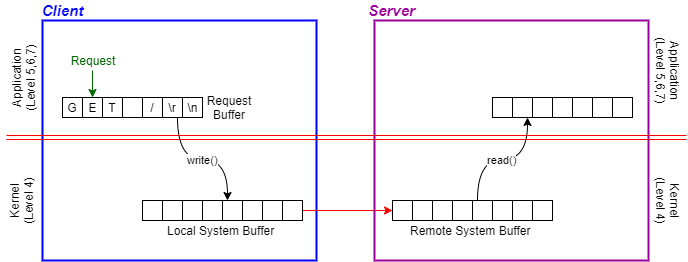
\includegraphics[scale=0.6]{Images/NetworkC/read_write1}\caption{\footnotesize{Request by the client.}}\label{rw1}
\end{figure}

\begin{figure}[h]
\centering
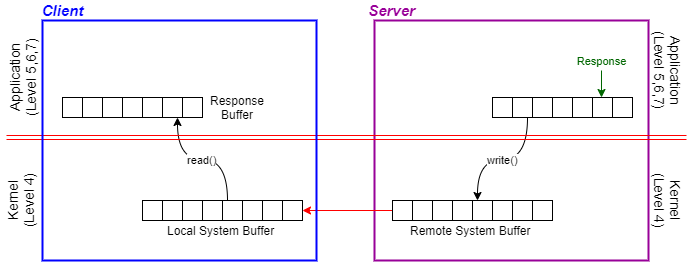
\includegraphics[scale=0.6]{Images/NetworkC/read_write2}\caption{\footnotesize{Response from the server.}}\label{rw2}
\end{figure}

\clearpage
\subsubsection{Client connection to google}
The following piece of code define a structure, used to connect to Google server. 
\lstinputlisting[caption={\footnotesize{web\_client.c}}, style=code, firstnumber=1, firstline=1, lastline=73, label=web_client, language=c]{../src/2_tcp/web_client.c}

The most important thing is that \textbf{socket()} is entry-point for level 4, but also \textbf{connect()} is the request to Kernel to extablish the connection.\\ \textbf{read()} and \textbf{write()} are system calls used respectively to obtain result(response) of a request and to generate request.\\ These function permit us to ask to lower level to do this things, without knowing content of system buffers (stream).

\section{UDP connection}
UDP connection is defined by type \textbf{SOCK\_DGRAM} as specified in Section \ref{socket}. It's used for application in which we use small packets and we want immediate feedback directly from application. It isn't reliable because it doesn't need confirmation in transport layer. It's used in Twitter application and in video streaming.  
\chapter{HTTP protocol}
HTTP protocol was presented for the first time in the RFC 1945 (Request for Comment).\\
The Hypertext Transfer Protocol (HTTP) is an application-level protocol with the lightness and speed necessary for distributed, collaborative, hypermedia information systems. It is a generic, stateless, object-oriented protocol which can be used for many tasks, such as name servers and distributed object management systems, through extension of its request methods (commands).\\
It's not the first Hypertext protocol in history because there was Hypertalk, made by Apple before. \\
A feature of HTTP is the typing of data representation, allowing systems to be built independently f the data being transferred. HTTP has been in use by the World-Wide Web global information initiative since 1990.

\section{Terminology}
\begin{itemize}
\item{\textbf{connection}\\
a transport layer virtual circuit established between two application programs for the purpose of communication.}
\item{\textbf{message}\\
the basic unit of HTTP communication, consisting of a structured sequence of octets matching the syntax defined in Section 4 and transmitted via the connection.}
\item{\textbf{request}\\
an HTTP request message.
}
\item{\textbf{response}\\
an HTTP response message.}
\item{\textbf{resource}\\
a network data object or service which can be identified by a URI.}
\item{\textbf{entity}\\
a particular representation or rendition of a data resource, or reply from a service resource, that may be enclosed within a request or response message. An entity consists of metainformation in the form of entity headers and content in the form of an entity body.}
\item{\textbf{client}\\
an application program that establishes connections for the purpose of sending requests.}
\item{\textbf{user agent}\\
the client which initiates a request. These are often browsers, editors, spiders (web-traversing robots), or other end user tools.}
\item{\textbf{server}\\
an application program that accepts connections in order to service requests by sending back responses.}
\item{\textbf{origin server}\\
the server on which a given resource resides or is to be created.}
\item{\textbf{proxy}\\
an intermediary program which acts as both a server and a client for the purpose of making requests on behalf of other clients. Requests are serviced internally or by passing them, with possible translation, on to other servers. A proxy must interpret and, if necessary, rewrite a request message before forwarding it.\\
Proxies are often used as client-side portals
through network firewalls and as helper applications for handling requests via protocols not implemented by the user agent.}
\item{\textbf{gateway}\\
a server which acts as an intermediary for some other server. Unlike a proxy, a gateway receives requests as if it were the origin server for the requested resource; the requesting client may not be aware that it is communicating with a gateway.\\
Gateways are often used as server-side portals through network firewalls and as protocol translators for access to resources stored on non-HTTP systems.}
\item{\textbf{tunnel}\\
a tunnel is an intermediary program which is acting as a blind relay between two connections. Once active, a tunnel is not considered a party to the HTTP communication, though the tunnel may have been initiated by an HTTP request. The tunnel ceases to exist when both ends of the relayed connections are closed.\\
Tunnels are used when a portal is necessary and the intermediary cannot, or should not, interpret the relayed communication.}
\item{\textbf{cache}\\
a program's local store of response messages and the subsystem that controls its message storage, retrieval, and deletion. A cache stores cachable responses in order to reduce the response time and network bandwidth consumption on future, equivalent requests. Any client or server may include a cache, though a cache cannot be used by a server while it is acting as a tunnel.}
\end{itemize}
Any given program may be capable of being both a client and a server; our use of these terms refers only to the role being performed by the program for a particular connection, rather than to the program's capabilities in general. Likewise, any server may act as an origin server, proxy, gateway, or tunnel, switching behavior based on the nature of each request.

\section{Basic rules}
The following rules are used throughout are used to describe the grammar used in the RFC 1945.
\begin{table}[h]
\centering
\footnotesize
\begin{tabular}{rl}
\textbf{OCTET =}& <any 8-bit sequence of data>\\
\textbf{CHAR =}& <any US-ASCII character (octets 0 - 127)>\\
\textbf{UPALPHA =}& <any US-ASCII uppercase letter "A".."Z">\\
\textbf{LOALPHA =}& <any US-ASCII lowercase letter "a".."z">\\
\textbf{ALPHA =}& UPALPHA | LOALPHA\\
\textbf{DIGIT =}& <any US-ASCII digit "0".."9">\\
\textbf{CTL =}& <any US-ASCII control character (octets 0 - 31) and DEL (127)>\\
\textbf{CR =}& <US-ASCII CR, carriage return (13)>\\
\textbf{LF =}& <US-ASCII LF, linefeed (10)>\\
\textbf{SP =}& <US-ASCII SP, space (32)>\\
\textbf{HT =}& <US-ASCII HT, horizontal-tab (9)>\\
\textbf{<"> =}& <US-ASCII double-quote mark (34)>\\
\end{tabular}
\end{table}

\section{Messages}
\subsection{Different versions of HTTP protocol}
\begin{itemize}
\item{\textbf{HTTP/0.9 Messages}\\
Simple-Request and Simple-Response do not allow the use of any header information and are limited to a single request method (GET).\\ Use of the Simple-Request format is discouraged because it prevents the server from identifying the media type of the returned entity.
\begin{center}
\begin{tabular}{c}
\begin{lstlisting}[linewidth=240pt, basicstyle=\footnotesize\sffamily,]
HTTP-message = Simple-Request | Simple-Response
\end{lstlisting}
\end{tabular}
\end{center}
\begin{center}
\begin{tabular}{c}
\begin{lstlisting}[linewidth=230pt, basicstyle=\footnotesize\sffamily,]
Simple-Request  = "GET" SP Request-URI CRLF


Simple-Response = [ Entity-Body ]
\end{lstlisting}
\end{tabular}
\end{center}
}
\item{\textbf{HTTP/1.0 Messages}\\
Full-Request and Full-Response use the generic message format of RFC 822 for transferring entities. Both messages may include optional header fields (also known as "headers") and an entity body. The entity body is separated from the headers by a null line (i.e., a line with nothing preceding the CRLF).
\begin{center}
\begin{tabular}{c}
\begin{lstlisting}[linewidth=230pt, basicstyle=\footnotesize\sffamily,]
HTTP-message = Full-Request | Full-Response
\end{lstlisting}
\end{tabular}
\end{center}
\begin{center}
\begin{tabular}{c}
\begin{lstlisting}[linewidth=340pt, basicstyle=\footnotesize\sffamily,]
Full-Request = Request-Line
               *(General-Header | Request-Header | Entity-Header)
               CRLF
               [Entity-Body]
               
               
Full-Response = Status-Line
                *(General-Header | Request-Header | Entity-Header)
                CRLF
                [Entity-Body]               
\end{lstlisting}
\end{tabular}
\end{center}
}
\end{itemize}

\subsection{Headers}
The order in which header fields are received is not significant. However, it is "good practice" to send General-Header fields first, followed by Request-Header or Response-Header fields prior to the Entity-Header fields.\\
Multiple HTTP-header fields with the same field-name may be present in a message if and only if the entire field-value for that header field is defined as a comma-separated list.
\begin{center}
\begin{tabular}{c}
\begin{lstlisting}[linewidth=260pt, basicstyle=\footnotesize\sffamily,]
HTTP-header = field-name ":" [ field-value ] CRLF
\end{lstlisting}
\end{tabular}
\end{center}

\subsection{Request-Line}
\begin{center}
\begin{tabular}{c}
\begin{lstlisting}[linewidth=320pt, basicstyle=\footnotesize\sffamily,]
Request-Line = Method SP Request-URI SP HTTP-Version CRLF

Method         = "GET" | "HEAD" | "POST" | extension-method

extension-method = token
\end{lstlisting}
\end{tabular}
\end{center}
The list of methods acceptable by a specific resource can change dynamically; the client is notified through the return code of the response if a method is not allowed on a resource.\\
Servers should return the status code 501 (not implemented) if the method is unrecognized or not implemented.

\subsection{Request-URI}
The Request-URI is a Uniform Resource Identifier and identifies the resource upon which to apply the request.
\begin{center}
\begin{tabular}{c}
\begin{lstlisting}[linewidth=190pt, basicstyle=\footnotesize\sffamily,]
Request-URI = absoluteURI | abs_path
\end{lstlisting}
\end{tabular}
\end{center}
The absoluteURI form is only allowed when the request is being made to a proxy. The proxy is requested to forward the request and return the response. If the request is GET or HEAD and a prior response is cached, the proxy may use the cached message if it passes any restrictions in the Expires header field.\\
Note that the proxy may forward the request on to another proxy or directly to the server specified by the absoluteURI. In order to avoid request loops, a proxy must be able to recognize all of its server names, including any aliases, local variations, and the numeric IP address.\\\\
The most common form of Request-URI is that used to identify a resource on an origin server or gateway. In this case, only the absolute path of the URI is transmitted.

\subsection{Request Header}
The request header fields allow the client to pass additional information about the request, and about the client itself, to the server.\\
These fields act as request modifiers, with semantics equivalent to the parameters on a programming language method (procedure) invocation.
\begin{center}
\begin{tabular}{c}
\begin{lstlisting}[linewidth=410pt, basicstyle=\footnotesize\sffamily,]
Request-Header = Authorization | From | If-Modified-Since | Referer | User-Agent
\end{lstlisting}
\end{tabular}
\end{center} 

\subsection{Status line}
\begin{center}
\begin{tabular}{c}
\begin{lstlisting}[linewidth=330pt, basicstyle=\footnotesize\sffamily,]
Status-Line = HTTP-Version SP Status-Code SP Reason-Phrase CRLF
\end{lstlisting}
\end{tabular}
\end{center}
\begin{table}[h]
\centering
\footnotesize
\begin{tabular}{|r|l|}
\multicolumn{2}{c}{\textbf{General Status code}}\\
\hline
\textbf{1xx: Informational} & {Not used, but reserved for future use}\\
\hline
\textbf{2xx: Success}&{The action was successfully received,}\\
\hline
& {understood, and accepted.}\\
\hline
\textbf{3xx: Redirection} & {Further action must be taken in order to}\\
&{complete the request}\\
\hline
\textbf{4xx: Client Error}&{The request contains bad syntax or cannot}\\
&{be fulfilled}\\
\hline
\textbf{5xx: Server Error}&{The server failed to fulfill an apparently}\\
&{valid request}\\
\hline
\end{tabular}
\end{table}
\begin{table}[h]
\centering
\footnotesize
\begin{tabular}{|r|l|}
\multicolumn{2}{c}{\textbf{Known service code}}\\
\hline
\textbf{200}&{OK}\\
\hline
\textbf{201}&{Created}\\
\hline
\textbf{202}&{Accepted}\\
\hline
\textbf{204}&{No Content}\\
\hline
\textbf{301}&{Moved Permanently}\\
\hline
\textbf{302}&{Moved Temporarily}\\
\hline
\textbf{304}&{Not Modified}\\
\hline
\textbf{400}&{Bad Request}\\
\hline
\textbf{401}&{Unauthorized}\\
\hline
\textbf{403}&{Forbidden}\\
\hline
\textbf{404}&{Not Found}\\
\hline
\textbf{500}&{Internal Server Error}\\
\hline
\textbf{501}&{Not Implemented}\\
\hline
\textbf{502}&{Bad Gateway}\\
\hline
\textbf{503}&{Service Unavailable}\\
\hline
\end{tabular}
\end{table}

\vspace{10cm}
\section{Examples}
The following pieces of code are examples of TCP client connection to \textbf{www.google.it}, using functions explained in Chapter \ref{networkC}.
\subsection{HTTP 0.9}
The following piece of code define a structure, used to connect to Google server. 

The most important thing is that \textbf{socket()} is entry-point for level 4, but also \textbf{connect()} is the request to Kernel to extablish the connection.\\ \textbf{read()} and \textbf{write()} are system calls used respectively to obtain result(response) of a request and to generate request.\\ These function permit us to ask to lower level to do this things, without knowing content of system buffers (stream). The second part is only used to read the input.

\subsection{HTTP 1.0}
The protocol has no mandatory headers to be added in the request field. This protocol is compliant with HTTP 0.9.
To keep the connection alive, "Connection" header with "keep-alive" as header field must be added to request message. The server, receiving the request, replies with a message with the same header value for "Connection".\\
This is used to prevent the closure of the connection, so if the client needs to send another request, he can use the same connection.
This is usually used to send many files and not only one.\\
The connection is kept alive until either the client or the server decides that the connection is over and one of them drops the connection. If the client doesn't send new requests to the server, the second one usually drops the connection after a couple of minutes.\\
The client could read the response of request, with activated keep alive option, reading only header and looking to "Content-length" header field value to understand the length of the message body. This header is added only if a request with keep-alive option is done.\\
This must be done because we can't look only to empty system stream, because it could be that was send only the response of the first request or a part of the response.\\
Otherwise, when the option keep alive is not used, the client must fix a max number of characters to read from the specific response to his request, because he doesn't know how many character compose the message body. If you make many requests to server without keep-alive option, the server will reply requests, after the first, with only headers but empty body.\\

\subsection{HTTP 1.1}
It has by default the option keep alive actived by default with respect to HTTP 1.0. It has the mandatory header "Host" followed by the hostname of the remote system to which the request or the response is sent. The body is organized in chunks, so we need the connection kept alive to manage future new chunks.\\
This is useful with dynamic pages, in which the server doesn't know the length of the stream in advance and can update the content of the stream during the extablished connection, sending a fixed amount of bytes to client. We can check if the connection is chunked oriented, looking for the header "Transfer-Encoding" with value "chunked".\\ 
Each connection is composed by many chunks and each of them is composed by chunk length followed by chunk body, except for the last one that has length 0 (see Figure \ref{chunked_body}). The following grammar represents how the body is organized:
\begin{center}
\begin{tabular}{c}
\begin{lstlisting}[linewidth=320pt, basicstyle=\footnotesize\sffamily,]
Chunked-Body   = *chunk
                 last-chunk
                 trailer
                 CRLF

chunk          = chunk-size [ chunk-extension ] CRLF
                 chunk-data CRLF

chunk-size     = 1*HEX
last-chunk     = 1*("0") [ chunk-extension ] CRLF

chunk-extension= *( ";" chunk-ext-name [ "=" chunk-ext-val ] )

chunk-ext-name = token
chunk-ext-val  = token | quoted-string
chunk-data     = chunk-size(OCTET)
trailer        = *(entity-header CRLF)
\end{lstlisting}
\end{tabular}
\end{center}

\begin{figure}[h]
\centering
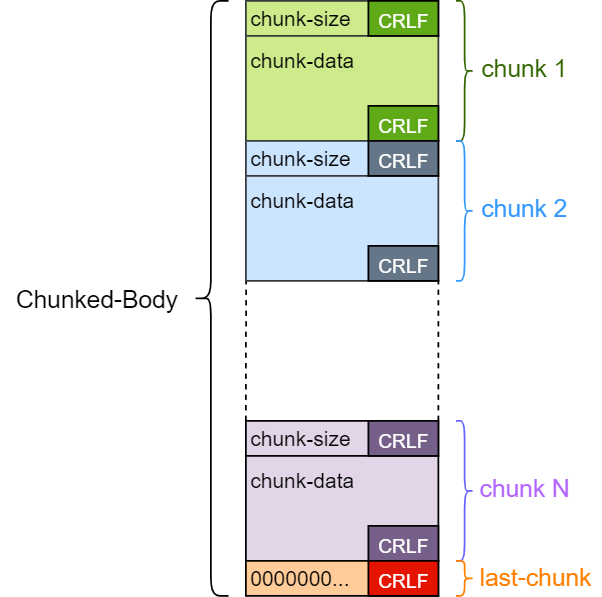
\includegraphics[scale=0.5]{Images/HTTP/Chunked-Body}\caption{\footnotesize{Chunked body.}}\label{chunked_body}
\end{figure}

\section{HTML}
The body of an HTTP request, it's often composed from the HTML related page. Each click, of a link inside the web page, generates a new request to the server with GET method.
\chapter{Code examples}
\section{Client HTTP 0.9}
\lstinputlisting[style=code, firstnumber=1, firstline=1, lastline=94, label=web_client, language=c]{../src/2_tcp/wc09.c}
\section{Client HTTP 1.0}
\lstinputlisting[style=code, firstnumber=1, firstline=1, lastline=193, label=web_client, language=c]{../src/2_tcp/wc10.c}
\section{Client HTTP 1.1}
\lstinputlisting[style=code, firstnumber=1, firstline=1, lastline=211, label=web_client, language=c]{../src/2_tcp/wc11.c}
\chapter{Shell}

\section{Commands}

\begin{table}[h]
\centering
\footnotesize
\begin{tabular}{|l|l|l|}
\hline
\multicolumn{2}{|l|}{\multirow{2}{*}{\textbf{man} man}}&{Shows info about man command and}\\
\multicolumn{2}{|l|}{} & {lists all the sections of the manual.}\\
\hline
\multicolumn{2}{|l|}{\textbf{strace} objFile} & {Lists all the system calls used in the program.}\\
\hline
\multicolumn{2}{|l|}{\textbf{gcc} -o objFile source \textbf{-v}} & {Lists all the path of libraries and headers used in creation of objFile.}\\
\hline
\multirow{3}{*}{\textbf{netstat}} & {-t} & {Lists all the active TCP connections showing domain names.}\\
\cline{2-3}
& {-u} & {Lists all the active UDP connections showing domain names.}\\
\cline{2-3}
& {-n} & {Lists all the active, showing IP and port numbers.}\\
\hline
\multicolumn{2}{|l|}{\textbf{nslookup} domain} & {Shows the IP address related to the domain (E.g. IP of www.google.it)}\\
\hline
\multicolumn{2}{|l|}{\multirow{5}{*}{\textbf{dig} @server name type}}&{DNS lookup utility.}\\
\multicolumn{2}{|l|}{}&{\textbf{server} name or IP address of the name server to query}\\
\multicolumn{2}{|l|}{}&{\textbf{name} name of the resource record that is to be looked up}\\
\multicolumn{2}{|l|}{}&{\textbf{type} type of query is required (ANY, A, MX, SIG, etc.)}\\
\multicolumn{2}{|l|}{}&{$\;\;\;\;\;\;\;\;\;\;$if no type is specified, A is performed by default}\\
\hline
\multicolumn{2}{|l|}{\multirow{2}{*}{\textbf{wc} [file]}} & {Prints in order newlines, words, and bytes (characters) counts for file}\\
\multicolumn{2}{|l|}{} & {if file not specified or equal to -, counts from stdin.}\\
\hline
\multicolumn{2}{|l|}{\multirow{2}{*}{\textbf{route} -n}} & {Show numerical addresses instead of trying to determine symbolic}\\
\multicolumn{2}{|l|}{} & {hostnames in routing table.}\\
\hline
\end{tabular}
\end{table}


\section{UNIX Files}\label{files}
\begin{table}[h]
\centering
\footnotesize
\begin{tabular}{|l|l|}
\hline
\textbf{/etc/hosts} & {Local resolution table.}\\
\hline
\multirow{2}{*}{\textbf{/etc/services}} & {List all the applications with their port}\\
& {and type of protocol (TCP/UDP).}\\
\hline
{\textbf{/etc/protocols}} & {Internet protocols.}\\
\hline
{\textbf{/usr/include/x86\_64-linux-gnu/bits/socket.h}} & {List all the protocol type possible for socket.}\\
\hline
{\textbf{/usr/include/x86\_64-linux-gnu/sys/socket.h}} & {Definition of struct sockaddr and specific ones.}\\
\hline
\end{tabular}
\end{table}

%\section{Usefull information about shell}
\end{document}